\documentclass[french]{beamer}
%\usepackage{listingsutf8}
%\usepackage[T1]{fontenc}
%\usepackage[utf8]{inputenc}
\usepackage{fontspec}
\usepackage[french]{babel}
\usepackage{amsmath, amssymb, mathrsfs}
\usepackage{graphicx}
\usepackage{listings}
\usepackage{tikz}
\usepackage{pgfplots}
\usepackage{epic, eepic}
\usepackage{fancybox}
\usepackage{array, multirow, tabularx}

\usetheme{Warsaw}
\mode<presentation>
\setbeamertemplate{navigation symbols}{}

\hypersetup{pdfpagemode=FullScreen, colorlinks=true,
  pdftitle={Présentation projet méthodes approchées.}, backref}

\title{Projet de méthodes approchées}

\institute{M1 informatique UM2}
\author{Dyce William, Loukil Amal, Ouazzani Sabrina}
\date{semestre 2 : 2011-2012}
\begin{document}

\begin{frame}
\titlepage
\end{frame}

\section{Introduction}

\begin{frame}
\frametitle{Problème}
\begin{itemize}
\item problèmes d'optimisation 
\begin{itemize}
\item[] $\nearrow$ problèmes faciles
\item[] $\searrow$ \fbox{problèmes NP-difficiles}
\end{itemize}
\item  $\Rightarrow$ méthodes exactes 
\begin{itemize}
\item[] $\nearrow$ programmation dynamique
\item[] $\searrow$ branch and bound
\end{itemize}


\item  $\Rightarrow$ méthodes approchées
\begin{itemize}
\item[] $\longrightarrow$ algorithmes d'approximation
\end{itemize}
\end{itemize}
\end{frame}

\begin{frame}
\frametitle{Table of Contents}
\begin{columns}
\begin{column}[]{5cm}
\tableofcontents
\end{column}
\begin{column}[]{4cm}
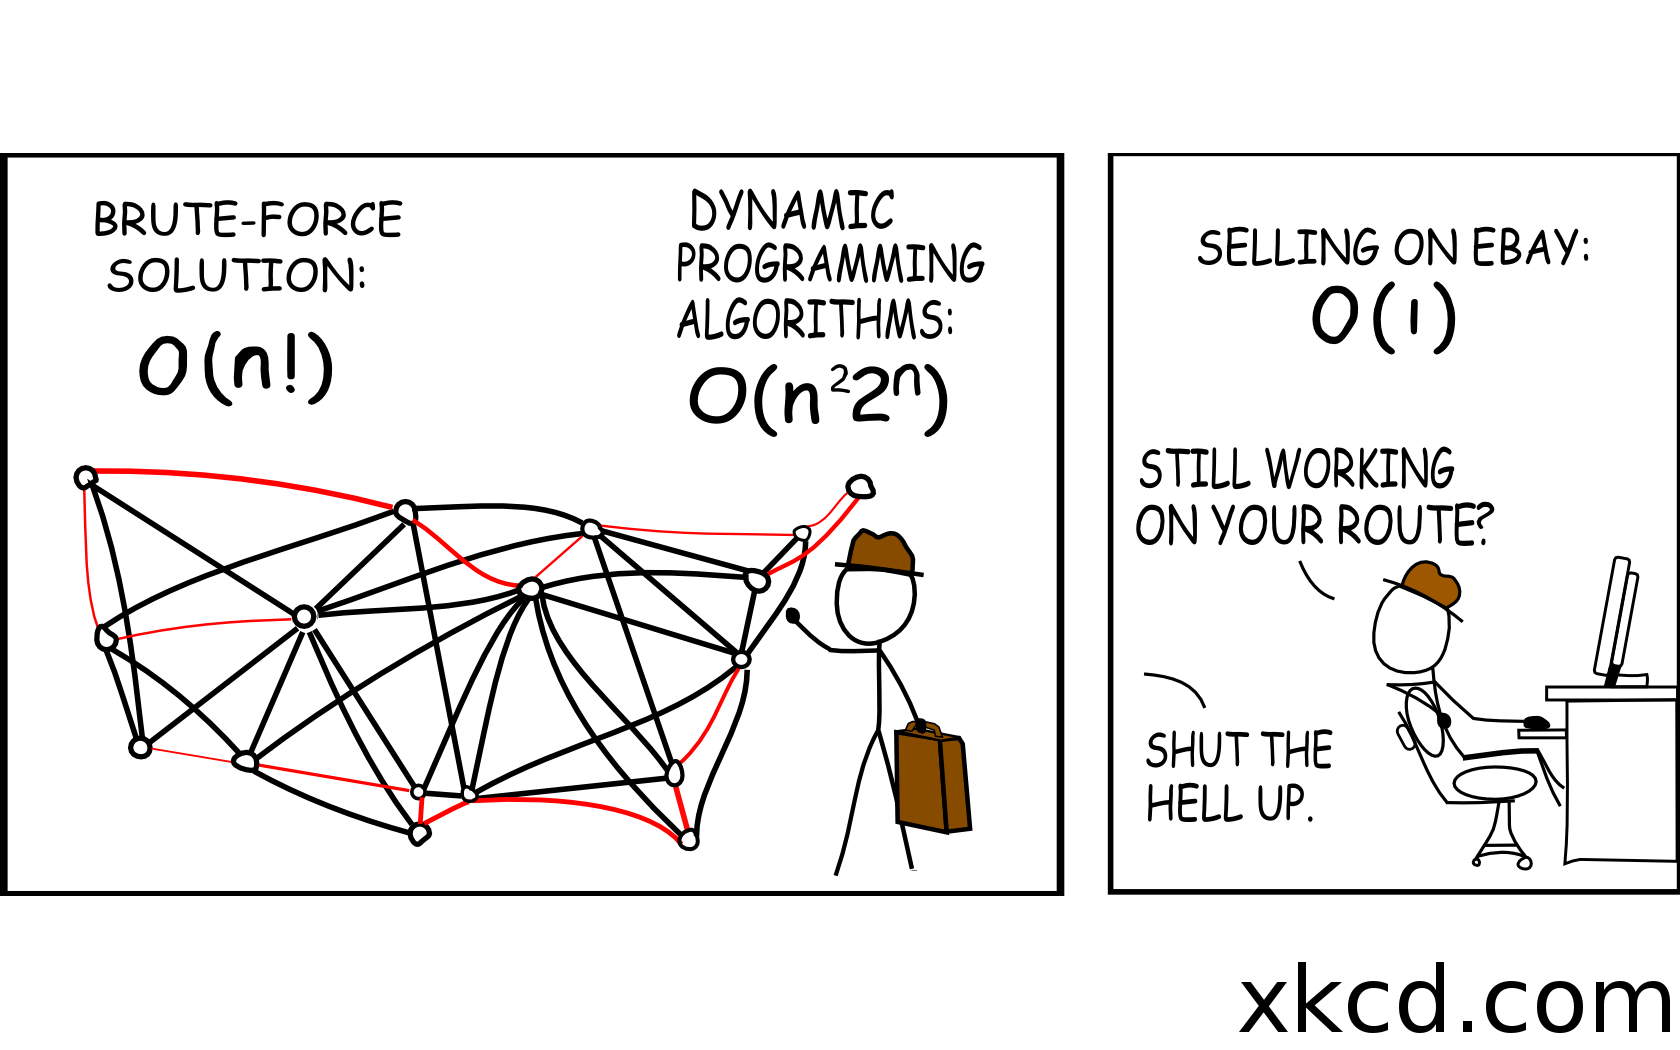
\includegraphics[height=3cm]{commerce.png}
\end{column}
\end{columns}
\end{frame}

\section{Programmation dynamique}

\begin{frame}
\frametitle{Outils}

\begin{block}{Programmation}
langage C
\end{block}

\begin{block}{Tests}
\begin{itemize}
\item tests unitaires
\item tests de temps d'exécution
\end{itemize}
\end{block}

\end{frame}

\begin{frame}
\frametitle{Partition}
\begin{alertblock}{Formules}
\begin{equation}
\begin{cases}
tab[0] = 1; \\
si ( tab[j] == 1 ) {
       tab[j + poids[i]] = 1;
     } \\
\end{cases}
\end{equation}
\end{alertblock}
\end{frame}

\begin{frame}
\frametitle{Partition}
\begin{block}{Jeux d'essai}

\end{block}
\end{frame}

\begin{frame}
\frametitle{Partition : courbe}

\end{frame}

\begin{frame}
\frametitle{Sac à dos}
\begin{alertblock}{Formules}
\begin{equation}
\begin{cases}
tab[0][w] = 0 \\
tab[i][j] = max(tab[i-1] [j], (tab[i-1] [j-poids[i]] + utilite[i])); \\
\end{cases}
\end{equation}
\end{alertblock}
\end{frame}

\begin{frame}
\frametitle{Sac à dos}
\begin{block}{Jeux d'essai}

\end{block}
\end{frame}

\begin{frame}
\frametitle{Sac à dos : courbe}
\end{frame}

\begin{frame}
\frametitle{Voyageur de commerce}
\begin{alertblock}{Formules}
\begin{equation}
\begin{cases}
C[S][i] = poids[0][i] \text{si S ne contient que $0$} \\
C[S][i] = min_{k \in S - \{ 0 \}} \{ C[S- \{ k \}][k] + poids[k][i]  \}
\end{cases}
\end{equation}
\end{alertblock}
\end{frame}

\begin{frame}
\frametitle{Voyageur de commerce}
\begin{block}{Jeux d'essai}
\end{block}
\end{frame}

\begin{frame}
\frametitle{Voyageur de commerce : courbe}
\end{frame}

\section{Branch and Bound TSP}

\begin{frame}
\frametitle{Outils}
\begin{block}{Langage}
\begin{itemize}
\item GLPK
\item langage C/C++
\end{itemize}
\end{block}
\end{frame}

\begin{frame}
\frametitle{Solution initiale}
\begin{itemize}
\item chaîne de poids le plus faible~;
\item voisinage 2--opt~;
\item voisinage 3--opt.
\end{itemize}
\end{frame}


\begin{frame}
\frametitle{Comparaisons}
\end{frame}

\begin{frame}
\frametitle{Complexité théorique}
\end{frame}

\begin{frame}
\frametitle{Jeux d'essais}
\end{frame}

\begin{frame}
\frametitle{Temps d'exécution}
\end{frame}

\section{Algorithme $\frac{3}{2}$ TSP}

\begin{frame}
\frametitle{Complexité théorique}
\end{frame}

\begin{frame}
\frametitle{Jeux d'essais}
\end{frame}

\begin{frame}
\frametitle{Temps d'exécution}
\end{frame}

\section{Comparaisons}

\begin{frame}
\frametitle{Jeux d'essais}

\end{frame}

\begin{frame}
\frametitle{Temps d'exécution}
\end{frame}

\section{Conclusion}
\begin{frame}

\end{frame}


\begin{frame}
\begin{center}
Merci pour votre attention.
\end{center}
\end{frame}

\end{document}
